\chapter{Robust covariance matrix estimation}
\label{chap:robust_vcv}

\section{Introduction}
\label{vcv-intro}

Consider (once again) the linear regression model
%
\begin{equation}
\label{eq:ols-again}
y = X\beta + u
\end{equation}
%
where $y$ and $u$ are $T$-vectors, $X$ is a $T \times k$ matrix of
regressors, and $\beta$ is a $k$-vector of parameters.  As is well
known, the estimator of $\beta$ given by Ordinary Least Squares (OLS)
is
%
\begin{equation}
\label{eq:ols-betahat}
\hat{\beta} = (X'X)^{-1} X'y
\end{equation}
%
If the condition $E(u|X) = 0$ is satisfied, this is an unbiased
estimator; under somewhat weaker conditions the estimator is biased
but consistent.  It is straightforward to show that when the OLS
estimator is unbiased (that is, when $E(\hat{\beta}-\beta) = 0$), its
variance is
%
\begin{equation}
\label{eq:ols-varb}
\mbox{Var}(\hat{\beta}) = 
  E\left((\hat{\beta}-\beta)(\hat{\beta}-\beta)'\right) 
  = (X'X)^{-1} X' \Omega X (X'X)^{-1}
\end{equation}
%
where $\Omega = E(uu')$ is the covariance matrix of the error terms.

Under the assumption that the error terms are independently and
identically distributed (iid) we can write $\Omega = \sigma^2 I$,
where $\sigma^2$ is the (common) variance of the errors (and the
covariances are zero).  In that case (\ref{eq:ols-varb}) simplifies to
the ``classical'' formula,
%
\begin{equation}
\label{eq:ols-classical-varb}
\mbox{Var}(\hat{\beta}) = \sigma^2(X'X)^{-1}
\end{equation}

If the iid assumption is not satisfied, two things follow.  First, it
is possible in principle to construct a more efficient estimator than
OLS---for instance some sort of Feasible Generalized Least Squares
(FGLS).  Second, the simple ``classical'' formula for the variance of
the least squares estimator is no longer correct, and hence the
conventional OLS standard errors---which are just the square roots of
the diagonal elements of the matrix defined by
(\ref{eq:ols-classical-varb})---do not provide valid means of
statistical inference.

In the recent history of econometrics there are broadly two approaches
to the problem of non-iid errors.  The ``traditional'' approach is to
use an FGLS estimator.  For example, if the departure from the iid
condition takes the form of time-series dependence, and if one
believes that this could be modeled as a case of first-order
autocorrelation, one might employ an AR(1) estimation method such as
Cochrane--Orcutt, Hildreth--Lu, or Prais--Winsten.  If the problem is
that the error variance is non-constant across observations, one might
estimate the variance as a function of the independent variables and
then perform weighted least squares, using as weights the reciprocals
of the estimated variances.

While these methods are still in use, an alternative approach has
found increasing favor: that is, use OLS but compute standard errors
(or more generally, covariance matrices) that are robust with respect
to deviations from the iid assumption.  This is typically combined
with an emphasis on using large datasets---large enough that the
researcher can place some reliance on the (asymptotic) consistency
property of OLS.  This approach has been enabled by the availability
of cheap computing power.  The computation of robust standard errors
and the handling of very large datasets were daunting tasks at one
time, but now they are unproblematic.  The other point favoring the
newer methodology is that while FGLS offers an efficiency advantage in
principle, it often involves making additional statistical assumptions
which may or may not be justified, which may not be easy to test
rigorously, and which may threaten the consistency of the
estimator---for example, the ``common factor restriction'' that is
implied by traditional FGLS ``corrections'' for autocorrelated errors.

James Stock and Mark Watson's \textit{Introduction to Econometrics}
illustrates this approach at the level of undergraduate instruction:
many of the datasets they use comprise thousands or tens of thousands
of observations; FGLS is downplayed; and robust standard errors are
reported as a matter of course.  In fact, the discussion of the
classical standard errors (labeled ``homoskedasticity-only'') is
confined to an Appendix.

Against this background it may be useful to set out and discuss all
the various options offered by gretl in respect of robust
covariance matrix estimation.  The first point to notice is that
gretl produces ``classical'' standard errors by default (in all
cases apart from GMM estimation).  In script mode you can get robust
standard errors by appending the \option{robust} flag to estimation
commands.  In the GUI program the model specification dialog usually
contains a ``Robust standard errors'' check box, along with a
``configure'' button that is activated when the box is checked.  The
configure button takes you to a configuration dialog (which can also
be reached from the main menu bar: Tools $\rightarrow$ Preferences
$\rightarrow$ General $\rightarrow$ HCCME).  There you can select from
a set of possible robust estimation variants, and can also choose to
make robust estimation the default.

The specifics of the available options depend on the nature of the
data under consideration---cross-sectional, time series or panel---and
also to some extent the choice of estimator.  (Although we introduced
robust standard errors in the context of OLS above, they may be used
in conjunction with other estimators too.)  The following three
sections of this chapter deal with matters that are specific to the
three sorts of data just mentioned.  Note that additional details
regarding covariance matrix estimation in the context of GMM are given
in chapter~\ref{chap:gmm}.

We close this introduction with a brief statement of what ``robust
standard errors'' can and cannot achieve.  They can provide for
asymptotically valid statistical inference in models that are
basically correctly specified, but in which the errors are not iid.
The ``asymptotic'' part means that they may be of little use in small
samples.  The ``correct specification'' part means that they are not a
magic bullet: if the error term is correlated with the regressors, so
that the parameter estimates themselves are biased and inconsistent,
robust standard errors will not save the day.


\section{Cross-sectional data and the HCCME}
\label{vcv-hccme}

With cross-sectional data, the most likely departure from iid errors
is heteroskedasticity (non-constant variance).\footnote{In some
  specialized contexts spatial autocorrelation may be an issue.  Gretl
  does not have any built-in methods to handle this and we will not
  discuss it here.}  In some cases one may be able to arrive at a
judgment regarding the likely form of the heteroskedasticity, and
hence to apply a specific correction.  The more common case, however,
is where the heteroskedasticity is of unknown form.  We seek an
estimator of the covariance matrix of the parameter estimates that
retains its validity, at least asymptotically, in face of unspecified
heteroskedasticity.  It is not obvious \textit{a priori} that this
should be possible, but \cite{white80} showed that
%
\begin{equation}
\label{eq:ols-varb-h}
\widehat{\mbox{Var}}_{\rm h}(\hat{\beta}) = 
       (X'X)^{-1} X' \hat{\Omega} X (X'X)^{-1}
\end{equation}
%
does the trick. (As usual in statistics we need to say ``under
certain conditions'', but the conditions are not very restrictive.)
$\hat{\Omega}$ is in this context a diagonal matrix, whose non-zero
elements may be estimated using squared OLS residuals.  White referred
to (\ref{eq:ols-varb-h}) as a heteroskedasticity-consistent covariance
matrix estimator (HCCME).

Davidson and MacKinnon (\citeyear{davidson-mackinnon04}, chapter 5)
offer a useful discussion of several variants on White's HCCME
theme. They refer to the original variant of
(\ref{eq:ols-varb-h})---in which the diagonal elements of
$\hat{\Omega}$ are estimated directly by the squared OLS residuals,
$\hat{u}^2_t$---as HC$_0$.  (The associated standard errors are often
called ``White's standard errors''.)  The various refinements of
White's proposal share a common point of departure, namely the idea
that the squared OLS residuals are likely to be ``too small'' on
average.  This point is quite intuitive.  The OLS parameter estimates,
$\hat{\beta}$, satisfy by design the criterion that the sum of squared
residuals,
%
\[
\sum \hat{u}^2_t = \sum \left( y_t - X_t \hat{\beta} \right)^2
\]
%
is minimized for given $X$ and $y$.  Suppose that $\hat{\beta} \neq
\beta$.  This is almost certain to be the case: even if OLS is not
biased it would be a miracle if the $\hat{\beta}$ calculated from any
finite sample were exactly equal to $\beta$.  But in that case the sum
of squares of the true, unobserved \textit{errors}, $\sum u^2_t = \sum
(y_t - X_t \beta)^2$ is bound to be greater than $\sum \hat{u}^2_t$.
The elaborated variants on HC$_0$ take this point on board as follows:
%
\begin{itemize}
\item HC$_1$: Applies a degrees-of-freedom correction, multiplying the
  HC$_0$ matrix by $T/(T-k)$.
\item HC$_2$: Instead of using $\hat{u}^2_t$ for the diagonal elements
  of $\hat{\Omega}$, uses $\hat{u}^2_t/(1-h_t)$, where
  $h_t = X_t(X'X)^{-1}X'_t$, the $t^{\rm th}$ diagonal element of the
  projection matrix $P_X$, which has the property that
  $P_X\cdot y = \hat{y}$.  The relevance of $h_t$ is that if the
  variance of all the $u_t$ is $\sigma^2$, the expectation of
  $\hat{u}^2_t$ is $\sigma^2(1-h_t)$, or in other words, the ratio
  $\hat{u}^2_t/(1-h_t)$ has expectation $\sigma^2$.  As Davidson and
  MacKinnon show, $0\leq h_t <1$ for all $t$, so this adjustment
  cannot reduce the the diagonal elements of $\hat{\Omega}$ and in
  general revises them upward.
\item HC$_3$: Uses $\hat{u}^2_t/(1-h_t)^2$.  The additional factor of
  $(1-h_t)$ in the denominator, relative to HC$_2$, may be justified
  on the grounds that observations with large variances tend to exert
  a lot of influence on the OLS estimates, so that the corresponding
  residuals tend to be under-estimated.  See Davidson and MacKinnon
  for a fuller explanation.
\item HC$_{3a}$: Implements the jackknife approach from
  \cite{mackinnon-white85}. (HC$_3$ is a close approximation of this.)
\end{itemize}

The relative merits of these variants have been explored by means of
both simulations and theoretical analysis.  Unfortunately there is not
a clear consensus on which is ``best''.  Davidson and MacKinnon argue
that the original HC$_0$ is likely to perform worse than the others;
nonetheless, ``White's standard errors'' are reported more often than
the more sophisticated variants and therefore, for reasons of
comparability, HC$_0$ is the default HCCME in gretl.

If you wish to use HC$_1$, HC$_2$, HC$_3$, or HC$_{3a}$ you can arrange
for this in either of two ways.  In script mode, you can do, for example,
%
\begin{code}
set hc_version 2
\end{code}
%
In the GUI program you can go to the HCCME configuration dialog, as
noted above, and choose any of these variants to be the default.


\section{Time series data and HAC covariance matrices}
\label{vcv-hac}

Heteroskedasticity may be an issue with time series data too but it
is unlikely to be the only, or even the primary, concern.  

One form of heteroskedasticity is common in macroeconomic time series
but is fairly easily dealt with.  That is, in the case of strongly
trending series such as Gross Domestic Product, aggregate consumption,
aggregate investment, and so on, higher levels of the variable in
question are likely to be associated with higher variability in
absolute terms.  The obvious ``fix'', employed in many
macroeconometric studies, is to use the logs of such series rather
than the raw levels.  Provided the \textit{proportional} variability
of such series remains roughly constant over time the log
transformation is effective.  

Other forms of heteroskedasticity may resist the log transformation,
but may demand a special treatment distinct from the calculation of
robust standard errors.  We have in mind here \textit{autoregressive
  conditional} heteroskedasticity, for example in the behavior of
asset prices, where large disturbances to the market may usher in
periods of increased volatility.  Such phenomena call for specific
estimation strategies, such as GARCH (see
chapter~\ref{chap:timeseries}).

Despite the points made above, some residual degree of
heteroskedasticity may be present in time series data: the key point
is that in most cases it is likely to be combined with serial
correlation (autocorrelation), hence demanding a special treatment.
In White's approach, $\hat{\Omega}$, the estimated covariance matrix
of the $u_t$, remains conveniently diagonal: the variances,
$E(u^2_t)$, may differ by $t$ but the covariances, $E(u_t u_s)$ for
$s \neq t$, are all zero.  Autocorrelation in time series data means
that at least some of the the off-diagonal elements of $\hat{\Omega}$
should be non-zero.  This introduces a substantial complication and
requires another piece of terminology: estimates of the covariance
matrix that are asymptotically valid in face of both
heteroskedasticity and autocorrelation of the error process are termed
HAC (heteroskedasticity- and autocorrelation-consistent).

The issue of HAC estimation is treated in more technical terms in
chapter~\ref{chap:gmm}.  Here we try to convey some of the intuition
at a more basic level.  We begin with a general comment: residual
autocorrelation is not so much a property of the data as a symptom of
an inadequate model.  Data may be persistent though time, and if we
fit a model that does not take this aspect into account properly we
end up with a model with autocorrelated disturbances.  Conversely, it
is often possible to mitigate or even eliminate the problem of
autocorrelation by including relevant lagged variables in a time
series model, or in other words, by specifying the dynamics of the
model more fully.  HAC estimation should not be seen as the first
resort in dealing with an autocorrelated error process.

That said, the ``obvious'' extension of White's HCCME to the case of
autocorrelated errors would seem to be this: estimate the off-diagonal
elements of $\hat{\Omega}$ (that is, the autocovariances,
$E(u_t u_s)$) using, once again, the appropriate OLS residuals:
$\hat{\omega}_{ts} = \hat{u}_t \hat{u}_s$.  This is basically right,
but demands an important amendment.  We seek a \textit{consistent}
estimator, one that converges towards the true $\Omega$ as the sample
size tends towards infinity.  This can't work if we allow unbounded
serial dependence.  A larger sample will enable us to estimate more of
the true $\omega_{ts}$ elements (that is, for $t$ and $s$ more widely
separated in time) but will not contribute ever-increasing information
regarding the maximally separated $\omega_{ts}$ pairs since the
maximal separation itself grows with the sample size.  To ensure
consistency we have to confine our attention to processes exhibiting
temporally limited dependence. In other words we cut off the
computation of the $\hat{\omega}_{ts}$ values at some maximum value of
$p = t-s$, where $p$ is treated as an increasing function of the
sample size, $T$, although it cannot increase in proportion to $T$.

The simplest variant of this idea is to truncate the computation at
some finite lag order $p$, where $p$ grows as, say, $T^{1/4}$.  The
trouble with this is that the resulting $\hat{\Omega}$ may not be a
positive definite matrix.  In practical terms, we may end up with
negative estimated variances.  One solution to this problem is offered
by The Newey--West estimator \citep{newey-west87}, which assigns
declining weights to the sample autocovariances as the temporal
separation increases.

To understand this point it is helpful to look more closely at the
covariance matrix given in (\ref{eq:ols-varb-h}), namely,
%
\[
(X'X)^{-1} (X' \hat{\Omega} X) (X'X)^{-1}
\]
%
This is known as a ``sandwich'' estimator.  The bread, which appears
on both sides, is $(X'X)^{-1}$.  This $k \times k$ matrix is also the
key ingredient in the computation of the classical covariance matrix.
The filling in the sandwich is
%
\[
\begin{array}{ccccc}
\hat{\Sigma} & = & X' & \hat{\Omega} & X \\
{\scriptstyle (k \times k)} & &
{\scriptstyle (k \times T)} & {\scriptstyle (T \times T)} & 
  {\scriptstyle (T \times k)}
\end{array}
\]
%
It can be proven that under mild regularity conditions
$T^{-1} \hat{\Sigma}$ is a consistent estimator of the long-run
covariance matrix of the random $k$-vector $x_t \cdot u_t$.

From a computational point of view it is neither necessary nor
desirable to store the (potentially very large) $T \times T$ matrix
$\hat{\Omega}$ as such.  Rather, one computes the sandwich filling by
summation as a weighted sum:
%
\[
\hat{\Sigma} = \hat{\Gamma}(0) + \sum_{j=1}^p w_j 
  \left(\hat{\Gamma}(j) + \hat{\Gamma}'(j) \right)
\]
%
where $w_j$ is the weight given to lag $j > 0$ and the $k \times k$
matrix $\hat{\Gamma}(j)$, for $j \geq 0$, is given by
\[
  \hat{\Gamma}(j) = \sum_{t=j+1}^T \hat{u}_t \hat{u}_{t-j}\, X'_t\,
  X_{t-j} ;
\]
that is, the sample autocovariance matrix of $x_t \cdot u_t$ at lag
$j$, apart from a scaling factor $T$.

This leaves two questions.  How exactly do we determine the maximum
lag length or ``bandwidth'', $p$, of the HAC estimator?  And how
exactly are the weights $w_j$ to be determined?  We will return to the
(difficult) question of the bandwidth shortly.  As regards the
weights, gretl offers three variants.  The default is the
Bartlett kernel, as used by Newey and West.  This sets
\[
w_j = \left\{ \begin{array}{cc}
     1 - \frac{j}{p+1} & j \leq p \\
     0 & j > p
     \end{array}
    \right.
\]
so the weights decline linearly as $j$ increases.  The other two
options are the Parzen kernel and the Quadratic Spectral (QS) kernel.
For the Parzen kernel,
\[
w_j = \left\{ \begin{array}{cc}
    1 - 6a_j^2 + 6a_j^3 & 0 \leq a_j \leq 0.5 \\
    2(1 - a_j)^3 & 0.5 < a_j \leq 1 \\
    0 & a_j > 1
    \end{array}
    \right.
\]
where $a_j = j/(p+1)$, and for the QS kernel,
\[
w_j = \frac{25}{12\pi^2 d_j^2} 
   \left(\frac{\sin{m_j}}{m_j} - \cos{m_j} \right)
\]
where $d_j = j/p$ and $m_j = 6\pi d_j/5$.  

Figure~\ref{fig:kernels} shows the weights generated by these kernels,
for $p=4$ and $j$ = 1 to 9.

\begin{figure}[htbp]
\caption{Three HAC kernels}
\label{fig:kernels}
\centering
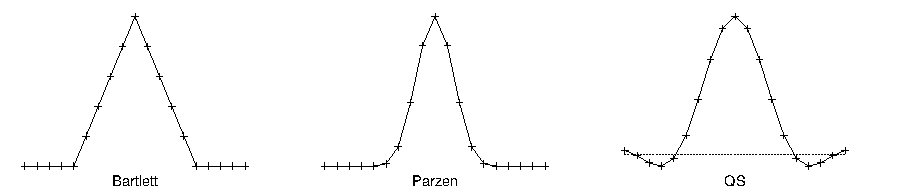
\includegraphics{figures/kernels}
\end{figure}

In gretl you select the kernel using the \texttt{set} command
with the \verb|hac_kernel| parameter:
%
\begin{code}
set hac_kernel parzen
set hac_kernel qs
set hac_kernel bartlett
\end{code}

\subsection{Selecting the HAC bandwidth}
\label{sec:hac-bw}

The asymptotic theory developed by Newey, West and others tells us in
general terms how the HAC bandwidth, $p$, should grow with the sample
size, $T$---that is, $p$ should grow in proportion to some
fractional power of $T$.  Unfortunately this is of little help to the
applied econometrician, working with a given dataset of fixed size.
Various rules of thumb have been suggested and gretl implements
two such.  The default is $p = 0.75 T^{1/3}$, as recommended by
\cite{stock-watson03}.  An alternative is $p = 4(T/100)^{2/9}$, as in
\cite{wooldridge-intro}.  In each case one takes the integer part of the
result.  These variants are labeled \texttt{nw1} and \texttt{nw2}
respectively, in the context of the \texttt{set} command with the
\verb|hac_lag| parameter.  That is, you can switch to the version
given by Wooldridge with
%
\begin{code}
set hac_lag nw2
\end{code}
%
As shown in Table~\ref{tab:haclag} the choice between \texttt{nw1} and
\texttt{nw2} does not make a great deal of difference.

\begin{table}[htbp]
  \centering
  \begin{tabular}{ccc}
    $T$ & $p$ (\texttt{nw1}) & $p$ (\texttt{nw2}) \\[4pt]
50& 	2& 	3 \\
100& 	3& 	4 \\
150& 	3& 	4 \\
200& 	4& 	4 \\
300& 	5& 	5 \\
400& 	5& 	5 \\
  \end{tabular}
\caption{HAC bandwidth: two rules of thumb}
\label{tab:haclag}
\end{table}

You also have the option of specifying a fixed numerical value for
$p$, as in

\begin{code}
set hac_lag 6
\end{code}

In addition you can set a distinct bandwidth for use with the
Quadratic Spectral kernel (since this need not be an integer).  For
example,
%
\begin{code}
set qs_bandwidth 3.5
\end{code}

\subsection{Prewhitening and data-based bandwidth selection}
\label{sec:hac-prewhiten}

An alternative approach is to deal with residual autocorrelation by
attacking the problem from two sides. The intuition behind the
technique known as \emph{VAR prewhitening} \citep{andrews92}
can be illustrated by a simple example.  Let $x_t$ be a sequence of
first-order autocorrelated random variables
%
\[
  x_t = \rho x_{t-1} + u_t
\]
%
The long-run variance of $x_t$ can be shown to be
%
\[
  V_{LR}(x_t) = \frac{V_{LR}(u_t)}{(1-\rho)^2}
\]
%
In most cases $u_t$ is likely to be less autocorrelated than $x_t$,
so a smaller bandwidth should suffice.  Estimation of $V_{LR}(x_t)$ can
therefore proceed in three steps: (1) estimate $\rho$; (2) obtain a
HAC estimate of $\hat{u}_t = x_t - \hat{\rho} x_{t-1}$; and (3)
divide the result by $(1-\rho)^2$.

The application of the above concept to our problem implies estimating
a finite-order Vector Autoregression (VAR) on the vector variables
$\xi_t = X_t \hat{u}_t$. In general the VAR can be of any order, but
in most cases 1 is sufficient; the aim is not to build a watertight
model for $\xi_t$, but just to ``mop up'' a substantial part of the
autocorrelation.  Hence, the following VAR is estimated
%
\[
  \xi_t = A \xi_{t-1} + \varepsilon_t
\]
%
Then an estimate of the matrix $X'\Omega X$ can be recovered via
\[
  (I- \hat{A})^{-1} \hat{\Sigma}_{\varepsilon} (I- \hat{A}')^{-1}
\]
where $\hat{\Sigma}_{\varepsilon}$ is any HAC estimator, applied to the VAR
residuals.

You can ask for prewhitening in gretl using
%
\begin{code}
set hac_prewhiten on
\end{code}
%
There is at present no mechanism for specifying an order other than 1
for the initial VAR.

A further refinement is available in this context, namely data-based
bandwidth selection.  It makes intuitive sense that the HAC bandwidth
should not simply be based on the size of the sample, but should
somehow take into account the time-series properties of the data (and
also the kernel chosen).  A nonparametric method for doing this was
proposed by \cite{newey-west94}; a good concise account of the
method is given in \cite{hall05}.  This option can be invoked in gretl
via
%
\begin{code}
set hac_lag nw3
\end{code}
%
This option is the default when prewhitening is selected, but you can
override it by giving a specific numerical value for \verb|hac_lag|.

Even the Newey--West data-based method does not fully pin down the
bandwidth for any particular sample.  The first step involves
calculating a series of residual covariances.  The length of this
series is given as a function of the sample size, but only up to a
scalar multiple---for example, it is given as $O(T^{2/9})$ for the
Bartlett kernel. Gretl uses an implied multiple of 1.

\subsection{Newey--West with missing values}
\label{sec:has-missvals}

If the estimation sample for a time-series model includes incomplete
observations---where the value of the dependent variable or one more
regressors is missing---the Newey--West procedure must be either
modified or abandoned, since some ingredients of the $\hat{\Sigma}$
matrix defined above will be absent. Two modified methods have been
discussed in the literature. \cite{parzen63} proposed what he called
Amplitude Modulation (AM), which involves setting the values of the
residual and each of the regressors to zero for the incomplete
observations (and then proceeding as usual). \cite{datta-du12} propose
the so-called Equal Spacing (ES) method: calculate as if the incomplete
observations did not exist, and the complete observations therefore
form an equally-spaced series. Somewhat suprisingly, it can be shown
that both of these methods have appropriate asymptotic properties;
see \cite{rho-vogelsang18} for further elaboration.

In gretl you can select a preferred method via one or other of these
commands:
\begin{code}
set hac_missvals es # ES, Datta and Du
set hac_missvals am # AM, Parzen
set hac_missvals off
\end{code}

The ES method is the default. The \texttt{off} option means that gretl
will refuse to produce HAC standard errors when the sample includes
incomplete observations: use this if you have qualms about the
modified methods.

\subsection{VARs: a special case}
\label{sec:hac-VARs}

A well-specified vector autoregression (VAR) will generally include
enough lags of the dependent variables to obviate the problem of
residual autocorrelation, in which case HAC estimation is
redundant---although there may still be a need to correct for
heteroskedasticity. For that reason plain HCCME, and not HAC, is the
default when the \option{robust} flag is given in the context of the
\cmd{var} command. However, if for some reason you need HAC you can
force the issue by giving the option \option{robust-hac}.

\subsection{Long-run variance}
\label{sec:lrvar}
% moved here from the "special functions" chapter in part I,
% where it really didn't belong

Let us expand a little on the subject of the long-run variance that
was mentioned above and the associated tools offered by gretl for
scripting. (You may also want to check out the reference for the
\texttt{lrcovar} function for the multivariate case.)  As is well
known, the variance of the average of $T$ random variables
$x_1, x_2, \ldots, x_T$ with equal variance $\sigma^2$ equals
$\sigma^2/T$ if the data are uncorrelated. In this case, the sample
variance of $x_t$ over the sample size provides a consistent
estimator.

If, however, there is serial correlation among the $x_t$s, the
variance of $\bar{X} = T^{-1} \sum_{t=1}^T x_t$ must be estimated
differently. One of the most widely used statistics for this purpose
is a nonparametric kernel estimator with the Bartlett kernel defined
as
\begin{equation}
  \label{eq:scalar-lrvar}
  \hat{\omega}^2(k) = T^{-1} \sum_{t=k}^{T-k} \left[ \sum_{i=-k}^k w_i (x_t -
  \bar{X}) (x_{t-i} - \bar{X}) \right] ,
\end{equation}
where the integer $k$ is known as the window size and the $w_i$ terms
are the so-called \emph{Bartlett weights}, defined as $w_i = 1 -
\frac{|i|}{k + 1}$. It can be shown that, for $k$ large enough,
$\hat{\omega}^2(k)/T$ yields a consistent estimator of the variance of
$\bar{X}$.

gretl implements this estimator by means of the function
\texttt{lrvar()}. This function takes one required argument, namely
the series whose long-run variance is to be estimated, followed by two
optional arguments. The first of these can be used to supply a value
for $k$; if it is omitted or negative, the popular choice $T^{1/3}$ is
used. The second allows specification of an assumed value for the
population mean of $X$, which then replaces $\bar{X}$ in the variance
calculation. Usage is illustrated below.
\begin{code}
# automatic window size; use xbar for mean
lrs2 = lrvar(x)
# set a window size of 12
lrs2 = lrvar(x, 12)
# set window size and impose assumed mean of zero
lrs2 = lrvar(x, 12, 0)
# impose mean zero, automatic window size
lrs2 = lrvar(x, -1, 0)
\end{code}

\section{Special issues with panel data}
\label{sec:vcv-panel}

Since panel data have both a time-series and a cross-sectional
dimension one might expect that, in general, robust estimation of the
covariance matrix would require handling both heteroskedasticity and
autocorrelation (the HAC approach).  In addition, some special features of
panel data require attention.
\begin{itemize}
\item The variance of the error term may differ across the
  cross-sectional units.
\item The covariance of the errors across the units may be non-zero in
  each time period.
\item If the ``between'' variation is not swept out, the errors may
  exhibit autocorrelation, not in the usual time-series sense but in
  the sense that the mean value of the error term may differ across
  units.  This is relevant when estimation is by pooled OLS.
\end{itemize}

Gretl currently offers three panel-specific covariance matrix
estimators in response to the \option{robust} option. These are
available for models estimated via fixed effects, random effects,
pooled OLS, and pooled two-stage least squares.  The default robust
estimator is that suggested by \cite{arellano03}, which is HAC
provided the panel is of the ``large $n$, small $T$'' variety (that
is, many units are observed in relatively few periods).  The Arellano
estimator involves clustering by the cross-sectional unit:
\[
\hat{\Sigma}_{\rm A} = 
\left(X^{\prime}X\right)^{-1}
\left( \sum_{i=1}^n X_i^{\prime} \hat{u}_i 
    \hat{u}_i^{\prime} X_i \right)
\left(X^{\prime}X\right)^{-1}
\]
where $X$ is the matrix of regressors (with the group means subtracted
in the case of fixed effects, or quasi-demeaned in the case of random
effects) $\hat{u}_i$ denotes the vector of residuals for unit $i$, and
$n$ is the number of such units.  \cite{cameron-trivedi05} make a
strong case for using this estimator; they note that the ordinary
White HCCME can produce misleadingly small standard errors in the
panel context because it fails to take autocorrelation into
account.\footnote{See also \cite{cameron-miller15} for a discussion of
  the Arellano-type estimator in the context of the random effects
  model.}  In addition \cite{stock-watson08} show that the White HCCME
is inconsistent in the fixed-effects panel context for fixed $T > 2$.

In cases where autocorrelation is not an issue the estimator proposed
by \cite{beck-katz95} and discussed by Greene (\citeyear{greene03},
chapter 13) may be appropriate.  This estimator, which takes into
account contemporaneous correlation across the units and
heteroskedasticity by unit, is
\[
\hat{\Sigma}_{\rm BK} = 
\left(X^{\prime}X\right)^{-1}
\left( \sum_{i=1}^n \sum_{j=1}^n \hat{\sigma}_{ij} X^{\prime}_iX_j \right)
\left(X^{\prime}X\right)^{-1}
\]
The covariances $\hat{\sigma}_{ij}$ are estimated via
\[
\hat{\sigma}_{ij} = \frac{\hat{u}^{\prime}_i \hat{u}_j}{T_i}
\]
where $T_i$ is the length of the time series for unit $i$.  Beck and
Katz call the associated standard errors ``Panel-Corrected Standard
Errors'' (PCSE).  This estimator can be invoked in gretl via the
command
%
\begin{code}
set panel_robust pcse
\end{code}
%
The Arellano default can be re-established via 
%
\begin{code}
set panel_robust arellano
\end{code}

The third panel-specific option is the spatial correlation consistent
(SCC) estimator developed by \cite{driscoll_kraay98}. This addresses
cross-sectional dependence of the disturbances as well as
heteroskedasticity and autocorrelation. Serial correlation is handled
in the manner of Newey--West and, unlike the Arellano estimator,
consistency is not limited to the ``small $T$'' case. The command to
select SCC is
\begin{code}
set panel_robust scc
\end{code}
An additional ``\texttt{set}'' variable is relevant when using this
estimator, namely \texttt{hac\_lag}, which governs the bandwidth of
the kernel employed in the Newey--West component as described in
section~\ref{sec:hac-bw} above. But note that in the SCC context only
the Bartlett kernel is supported, and neither prewhitening nor
data-based bandwidth selection are available.  So the applicable
\texttt{hac\_lag} variants are just \texttt{nw1}, \texttt{nw2} or a
user-specified maximum (integer) lag. To replicate results from the
\texttt{xtscc} command for \textsf{Stata} \citep{hoechle07} the
\texttt{nw2} variant should be selected.

Note that regardless of the \verb|panel_robust| setting, the robust
estimator is not used unless the \option{robust} flag is given with
the estimation command (or the ``Robust'' box is checked in the
graphical interface). For some further remarks on the panel case, the
following section.

\section{The cluster-robust estimator}
\label{sec:vcv-cluster}

One further variance estimator is available in gretl, namely the
``cluster-robust'' estimator. This may be appropriate (for
cross-sectional data, mostly) when the observations naturally fall
into groups or clusters, and one suspects that the error term may
exhibit dependency within the clusters and/or have a variance that
differs across clusters. Such clusters may be binary (e.g.\ employed
versus unemployed workers), categorical with several values (e.g.\
products grouped by manufacturer) or ordinal (e.g.\ individuals with
low, middle or high education levels). 

For linear regression models estimated via least squares the cluster
estimator is defined as
\[
\hat{\Sigma}_{\rm C} = \left(X'X\right)^{-1} 
  \left(\sum_{j=1}^m X_j'\hat{u}_j \hat{u}_j' X_j\right)
  \left(X'X\right)^{-1}
\]
where $m$ denotes the number of clusters, and $X_j$ and $\hat{u}_j$
denote, respectively, the matrix of regressors and the vector of
residuals that fall within cluster $j$. As noted above, the Arellano
variance estimator for panel data models is a special case of this,
where the clustering is by panel unit.

For models estimated by the method of Maximum Likelihood (in which
case the standard variance estimator is the inverse of the negative
Hessian, $H$), the cluster estimator is
\[
\hat{\Sigma}_{\rm C} = H^{-1} \left(\sum_{j=1}^m G_j' G_j\right)
  H^{-1}
\]
where $G_j$ is the sum of the ``score'' (that is, the derivative of
the loglikelihood with respect to the parameter estimates) across the
observations falling within cluster $j$.

It is common to apply a degrees of freedom adjustment to these
estimators (otherwise the variance may appear misleadingly small in
comparison with other estimators, if the number of clusters is small).
In the least squares case the factor is $(m/(m-1)) \times
(n-1)/(n-k)$, where $n$ is the total number of observations and $k$ is
the number of parameters estimated; in the case of ML estimation the
factor is just $m/(m-1)$.

\subsection{Availability and syntax}

The cluster-robust estimator is currently available for models
estimated via OLS and TSLS, and also for most ML estimators other than
those specialized for time-series data: binary logit and probit,
ordered logit and probit, multinomial logit, Tobit, interval
regression, biprobit, count models and duration models. Additionally,
the same option is available for generic maximum likelihood estimation
as provided by the \cmd{mle} command (see chapter \ref{chap:mle} for
more details).

The standard syntax is that you give the option flag \option{cluster=}
followed by the name of the series to be used to define the clusters,
as in
%
\begin{code}
ols y 0 x1 x2 --cluster=cvar
\end{code}
%
The specified clustering variable must (a) be defined (not missing) at
all observations used in estimating the model and (b) take on at least
two distinct values over the estimation range. The clusters are
defined as sets of observations having a common value for the
clustering variable. It is generally expected that the number of
clusters is substantially less than the total number of observations.

In the case of panel data, the \option{cluster} option can be used to
impose clustering by time period, or by a selected cross-sectional
characteristic. (Recall from the discussion above that the default
action of the \option{robust} option is to cluster by panel unit, so
if that is what you want the \option{cluster} option is not required.)

To invoke clustering by period the recommended form is
\verb|--cluster=$time|, where \verb|$time| is taken as a keyword
rather than the name of a series.\footnote{Letting gretl identify the
  periods is more efficient that specifying a series to that effect.}
Another plausible case for explicit use of clustering arises if the
dataset contains a series that identifies a set of groups into which
the panel units fall---for example, the panel units are individuals
but you know which individuals are members of which household, or the
panel units are counties but you know in which state each county is
located. Then you may wish to cluster at the group level, as in
\begin{code}
panel ... --cluster=household
# OR
panel ... --cluster=state
\end{code}
In these cases, of course, the parameter to \option{cluster} must be
the name of a series that does the job, providing a unique identifier
for each of the groups.

In the case of panel data only, two-way clustering is also supported.
For example, one might cluster by cross-sectional unit and
time-period, hence allowing for dependence of the disturbance term
both within unit and within period. But note that if a categorical
variable \texttt{C1} is nested within a more highly aggregated one,
\texttt{C2}, then two-way clustering is not called for since it
amounts to clustering on \texttt{C2} alone. The syntax for the two-way
case is on the following pattern
\begin{code}
panel ... --cluster=cvar1,cvar2
\end{code}
where two comma-separated terms are given (with no intervening
spaces). These terms can be the names of existing series, or the
accessors \verb|$time| and \verb|$unit| may be used to indicate
unique identifiers for time periods and cross-sectional units,
respectively.

The precise magnitude of standard errors produced in case of
cluster-robust estimation depends on whether a degrees of freedom
adjustment is applied, and if so on how exactly the adjustment is
calculated---a matter which is somewhat debatable. The default
procedure in gretl is that of \cite{CGM2011}. That is, we apply an
adjustment factor equal to
\[
  \frac{c}{c-1} \times \frac{n}{n-k}
\]
where $c$ is the number of clusters, $n$ is the total number of
observations, and $k$ is the number of parameters estimated. Results
then agree with \textsf{Stata}'s \texttt{xtreg} command and also the
\texttt{cgmreg} command made available by Colin Cameron.\footnote{As
  of 2023-10-12 this is available via
  \url{https://cameron.econ.ucdavis.edu/research/cgmreg.ado}.}  To
produce clustered standard errors in agreement with the popular
contributed \textsf{Stata} command \texttt{xtivreg2} it is necessary
to suppress this adjustment: append the \option{no-df-corr} option to
the \texttt{panel} command.

%%% Local Variables: 
%%% mode: latex
%%% TeX-master: "gretl-guide"
%%% End: 
